\chapter{Regresiones lineales}

En esta unidad, trataremos con una técnica básica de modelación predictiva llamada \emph{regresión lineal}, la cuál permite crear un modelo a partir de una base de datos histórica.


Nuestro propósito es entender las matemáticas detrás de la regresión lineal e ilustrar sus resultado a través de su implementación en varias bases de datos.

\paragraph{Mapa de ruta}
\begin{itemize}
 \item Las matemáticas detrás de la regresión lineal.
 \item Implementación de la regresión lineal con Python.
 \item Interpretación de los parámetros resultantes.
 \item Validación del modelo.
 \item Manejo de Problemas relacionados con regresión lineal.
\end{itemize}


\paragraph{Modelos matemáticos}
Un \emph{modelo matemático/estadístico/predictivo} es una ecuación matemática que consiste en \emph{entradas} que producen \emph{salidas} cuando el valor de las variables entrantes se introduce en el modelo.

\paragraph{Ejemplo}
Por ejemplo, supongamos que el precio $P$ de una casa es \emph{linealmente dependiente} en su tamaño $S$, comodidades $A$ y disponibilidad de transporte $T$.



La ecuación correspondiente sería
\begin{align}
 P = a_{1}\times S+ a_{2} \times A + a_{3} \times T
\end{align}



Esta ecuación es llamado el \emph{modelo} y los coeficientes $a_{1},a_{2},a_{3}$ son sus parámetros.



La variable $P$ es resultado predicho, mientras que $S,A,T$ con las variables de entrada, que son datos conocidos.


Sin embargo, los parámetros $a_{i}$ deben ser estimados a partir de los datos históricos.


Una vez que estos parámetros son determinados, el modelo está listo para ser problemaado.


\section{Entendiendo las matemáticas detrás de la regresión lineal}

Supongamos que tenemos una base de datos hipotética que contiene la información acerca del costo (en unidades de $\$10000$) de varias casas y sus respectivos tamaños (en pies cuadrados $ft^{2}$).


\begin{center}
\begin{tabular}{|l|l|}\hline
Tamaño & Costo\\\hline
1500 & 45\\\hline
1200 & 38\\\hline
1700 & 48\\\hline
800 & 27\\\hline
\end{tabular}
\end{center}



En este caso, el costo es la variable de salida, mientras que el tamaño es la variable de entrada. 

La entrada y la salida generalmente se denotan por $X$ y $Y$, respectivamente.


En el caso de la regresión lineal, supondremos que el costo $Y$ es una función lineal de tamaño $X$ y para estimar $Y,$ proponemos el modelo \begin{align}
 Y_{e} = \a + \beta X ,
\end{align}
donde $Y_{e}$ es el \emph{valor estimado} de $Y$ con base en nuestra ecuación lineal.


 \begin{rem}
  El propósito de la regresión lineal es encontrar valores $\alpha, \beta$ estadísticamente significativos, que \emph{minimicen} la diferencia entre $Y$ y $Y_{e}.$
 \end{rem}



En el caso de nuestro ejemplo, si encontramos los valores de $\a=2$ y $\beta=0.03,$ entonces la ecuación será
\begin{align}
 Y_{e}= 2 + 0.03 X.
\end{align}


Usando esta ecuación, podemos estimar el costo una casa de cualquier tamaño.  Por ejemplo, para una casa de $900 ft^{2}$, el costo será
\begin{align}
 Y_{e}= 2 + 0.03(900)= 29 .
\end{align}


La siguiente pregunta que nos haremos es como estimar $\a$ y $\beta.$  Para esto usaremos un método llamado suma de  \emph{mínimos cuadrados} para la diferencia entre $Y$ y $Y_{e},$ que representaremos como
\begin{align}
 \ep = Y-Y_{e}.
\end{align}

 

Nuestro objetivo es minimizar
 \begin{align}
  \sum \ep^{2} & = \sum \left( Y-Y_{e} \right)^{2}\\
  &= \sum \left( Y - \left( \a+\beta X \right) \right)^{2}
 \end{align}
respecto de los parámetros $\a, \beta.$


Utilizando un poco de cálculo, se puede demostrar que los valores de los parámetros que minimizan la suma anterior son
\begin{align}
\label{beta}
\beta &= \dfrac{\sum \left( x-\bar{x} \right)\left( y-\bar{y} \right)}{\sum\left( x-\bar{x} \right)^{2}}\\
\label{alfa}
\a &= \bar{y}-\beta\times \bar{x}
\end{align}

% \part{NO BORRAR}
% \section{Recursos}
% \paragraph{analisisPredictivo}
% El repositorio con los scripts de \texttt{Python 3} de esta presentación los puede encontrar en \href{https://github.com/julihocc/ulsaPye/tree/master/analisisPredictivo}{https://github.com/julihocc/ulsaPye/tree/master/analisisPredictivo}
% 
% [t, ]
% \frametitle{Referencias}
% \nocite{*}
% \betaibliographystyle{amsalpha}
% \betaibliography{ulsaPye}
% 
\section{Regresión lineal usando datos simulados}

Para propósitos de regresión lineal, escribimos $Y_{e}=\a+\beta X,$ aunque $Y$ rara vez será lineal y podría tener un componente de error o residual, y en ese caso escribimos
\begin{align}
 Y=\a + \beta X + K.
\end{align}


En la ecuación anterior, $K$ es el error, el cuál es una variable aleatoria que supondremos está normalmente distribuida.


Simulemos los datos para $X$ y $Y$ y tratemos de observar como es que los valores estimados $\left( Y_{e} \right)$ difieren del valor real $\left( Y \right)$.


Para $X,$ generamos 100 números aleatorios normalmente distribuidos con media $1.5$ y desviación estándar $2.5$ (pero usted puede tomar otro par de números y experimentar.)


\paragraph{Consideraciones}
\begin{enumerate}
 \item Para el valor $(Y_{e}),$ supondremos una ordenada al origen $\a=2$ y una pendiente $\beta=0.3$. 

 \item
Posteriormente, calcularemos los valores óptimos de $\a$ y $\beta$, usando los datos simulados y veremos como cambia la eficacia del modelo.

\item
Para el valor actual $Y$, adicionamos un término residual, que no es otra cosa que una variable normalmente distribuida con media $\mu=0$ y desviación estándar de $\sigma=0.5$.
\end{enumerate}


[,]{\texttt{fittingLinearRegression.py}}
\begin{lstlisting}[language=Python]
import pandas as pd
import numpy as np

np.random.seed(1234)

x=2.5*np.random.randn(100)+1.5
res=.5*np.random.randn(100)+0
ypred=2+.3*x
yact=2+.3*x+res
xlist=x.tolist()
ypredlist=ypred.tolist()
yactlist=yact.tolist()
df=pd.DataFrame({'Input_Variable(X)':xlist,'Predicted_Output(ypred)':ypredlist,'Actual_Output(yact)':yactlist})
print(df.head())


import matplotlib.pyplot as plt

% x=2.5*np.random.randn(100)+1.5
% res=.5*np.random.randn(100)+0
% ypred=2+.3*x
% yact=2+.3*x+res

ymean=np.mean(yact)
yavg=[ymean for i in range(1,len(xlist)+1)]

plt.plot(x,ypred)
plt.plot(x,yact,'ro')
plt.plot(x,yavg)
plt.title('Actual vs Predicted')
\end{lstlisting}

[,]{} \tiny
\begin{lstlisting}[language=Python]
   Actual_Output(yact)  Input_Variable(X)  Predicted_Output(ypred)
0             2.949179           2.678588                 2.803576
1             1.840035          -1.477439                 1.556768
2             3.776326           5.081767                 3.524530
3             2.358159           0.718370                 2.215511
4             2.151703          -0.301472                 1.909558
\end{lstlisting}


\begin{center}
 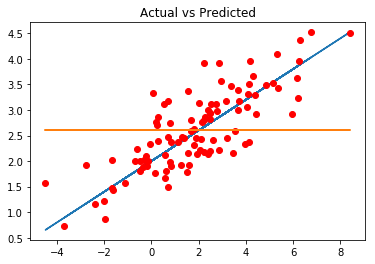
\includegraphics[width=10cm,keepaspectratio=true]{./images/actualVsPredicted.png}
 % actualVsPredicted.png: 0x0 pixel, 300dpi, 0.00x0.00 cm, bb=
\end{center}



En la gráfica anterior, la linea horizontal representa la \emph{media} de los datos.


En caso de que no tuviéramos algún otro modelo predictivo, nuestra mejor elección sería la \emph{media aritmética}.


Otro punto para pensar es en como juzgar la eficiencia de nuestro modelos. 

Si usted pasa cualquier dato conteniendo dos variables, una de entrada y otra de salida, el programa de estadística generara algunos valores $\a,\beta.$



¿Pero cómo entender que esos valores que se nos están dando son un buen modelo?

\paragraph{Suma de Cuadrados Total}
\begin{align}
 SST = \sum\left( Y_{i}-\bar{Y} \right)^{2}
\end{align}

donde $\bar{Y}$ es el valor promedio de $Y_{1}, Y_{2},...$, los valores reales de $Y.$


\paragraph{Suma de Cuadrados de Regresión}

\begin{align}
 SSR = \sum\left( Y_{e,i}-\bar{Y} \right)^{2}
\end{align}
donde $\bar{Y}$ es el valor promedio de $Y_{1}, Y_{2},...$, los valores reales de $Y,$ mientras que $Y_{e,i}$ son los valores predichos por el modelos para cada $Y_{i}.$


\paragraph{Suma de Cuadrados de Diferencia}
\begin{align}
 SSD = \sum\left( Y_{i}-Y_{e,i} \right)^{2}
\end{align}



Recordemos que $Y_{e}=\a + \beta X$, con $\beta$ definida por \eqref{beta} y $\a$ por \eqref{alfa}.



Utilizando estas identidad se puede demostrar que
\begin{align}
 SST = SSR +SSD.
\end{align}



\begin{itemize}
 \item $SSR$: diferencia explicada por el modelo;
 \item $SSD$: diferencia no explicada por el modelo;
 \item $SST$: error total.
\end{itemize}




\begin{rem}
 Entre mayor sera la proporción de $SSR:SST$, mejor será el modelo.
\end{rem}


\paragraph{Coeficiente de determinación}
\texttt{R-cuadrado: }
\begin{align}
 R^{2}=\dfrac{SSR}{SST}
\end{align}


Como $SSR\leq SST,$ entonces $0\leq R^{2} \leq 1$, y entre más cercano sea a $1$ mejor será el modelo.



$R^{2}$ es un buen indicador de que una regresión lineal será efectiva.


En el script \texttt{fittingLinearRegression.py}, podemos agregar el siguiente pedazo de código para calcular el valor $R^{2}$.

[,]{\texttt{rCuadrada.py}}
\begin{lstlisting}[language=Python]
df['SSR']=(df['Predicted_Output(ypred)']-ymean)**2
df['SST']=(df['Actual_Output(yact)']-ymean)**2
SSR=df.sum()['SSR']
SST=df.sum()['SST']
SSR/SST
\end{lstlisting}


El valor obtenido es $a\approx 0.65$, que es algo bueno. Sin embargo, los valores $\a=2, \beta=0.3$ para $Y_{e}$ pueden que no sean los mejores.

\section{Encontrando el valor optimo de los coeficientes de una regresión lineal}

Regresemos a nuestro marco de datos \texttt{df}. La columna \texttt{Input\_Variable(X)} es la variable predictora. 
La variable \texttt{Actual\_Output(yact)}, como su nombre lo siguiere, es la variable de salida real.


Utilizando estas dos variables, podemos calcular los valores de $\a$ y $\beta$ de acuerdo a las fórmulas \eqref{alfa} y \eqref{beta}.  En el siguiente script, implementaremos estas fórmulas para obtener un modelo optimo de regresión lineal.

[,]{\texttt{optimalValue.py}}
\begin{lstlisting}[language=Python]
#!/usr/bin/env python3
# -*- coding: utf-8 -*-
"""
Created on Mon Oct 23 00:37:36 2017

@author: jdk2py
"""

import pandas as pd
import numpy as np

np.random.seed(1234)

x=2.5*np.random.randn(100)+1.5
res=.5*np.random.randn(100)+0
ypred=2+.3*x
yact=2+.3*x+res
xlist=x.tolist()
ypredlist=ypred.tolist()
yactlist=yact.tolist()
df=pd.DataFrame({'Input_Variable(X)':xlist,'Predicted_Output(ypred)':ypredlist,'Actual_Output(yact)':yactlist})

ymean=np.mean(yact)
yavg=[ymean for i in range(1,len(xlist)+1)]

import matplotlib.pyplot as plt

xmean=np.mean(df['Input_Variable(X)'])
ymean=np.mean(df['Actual_Output(yact)'])
df['betan']=(df['Input_Variable(X)']-xmean)*(df['Actual_Output(yact)']-ymean)
df['xvar']=(df['Input_Variable(X)']-xmean)**2
betan=df.sum()['betan']
betad=df.sum()['xvar']
beta=betan/betad
alpha=ymean-beta*xmean
print(beta,alpha)

df['ymodel']=beta*df['Input_Variable(X)']+alpha

df['SSR']=(df['ymodel']-ymean)**2
df['SST']=(df['Actual_Output(yact)']-ymean)**2
SSR=df.sum()['SSR']
SST=df.sum()['SST']
R2 = SSR/SST

print(df.head())

plt.plot(x,ypred)
plt.plot(x,df['ymodel'], "b")
plt.plot(x,yact,'ro')
plt.plot(x,yavg)
plt.title('Actual vs Predicted vs Model')
\end{lstlisting}

[,]{}
\tiny
\begin{lstlisting}[language=Python]
   Actual_Output(yact)  Input_Variable(X)  Predicted_Output(ypred)     betan  \
0             2.949179           2.678588                 2.803576  0.543137
1             1.840035          -1.477439                 1.556768  1.873530
2             3.776326           5.081767                 3.524530  4.629773
3             2.358159           0.718370                 2.215511  0.080941
4             2.151703          -0.301472                 1.909558  0.565934

        xvar    ymodel       SSR       SST
0   1.189860  2.796261  0.119028  0.247926
1   9.395573  1.481781  0.939885  0.373592
2  12.207943  3.556345  1.221220  1.755808
3   0.755875  2.176277  0.075614  0.008667
4   3.569275  1.853719  0.357052  0.089733
\end{lstlisting}


\begin{center}
 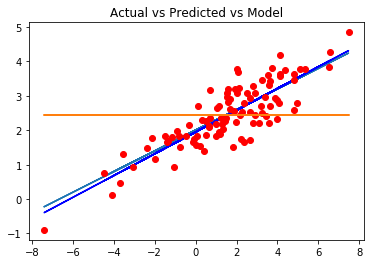
\includegraphics[width=10cm,keepaspectratio=true]{./images/optimalValue.png}
 % optimalValue.png: 0x0 pixel, 300dpi, 0.00x0.00 cm, bb=
\end{center}



Además del estadístico $R^{2}$, hay otras estadísticos y parámetros que uno necesita
mira para hacer lo siguiente:


\begin{enumerate}
\item Seleccionar algunas variables y deseche otras para el modelo.


\item Evaluar la relación entre el predictor y la variable de salida y verificar


si una variable de predicción es significativa en el modelo o no.
\item Calcular el error en los valores predichos por el modelo seleccionado.
\end{enumerate}




Veamos ahora algunas de los estadísticos que ayudan a abordar los Problemas
discutido anteriormente.

[]{Valor-$p$}
Es importante notar que al calcular los valores de $\a$ y $\beta,$ obtenemos estimados y no son exactos. Necesitamos demostrar su significación estadística usando una prueba de hipótesis.


La prueba de hipotética es acerca si el valor $\beta$ es diferente de cero o no. En otras palabras, si existe la correlación necesaria entre $X$ y $Y$. De haberla, $\beta \neq 0$.


En la ecuación $y = \a + \beta x,$ si hacemos $\beta=0,$ no existirá correlación entre $x$ y $y$. Entonces la prueba de hipótesis se define como
\begin{align}
 \texttt{Hipótesis Nula }H_{0}:\beta=0 \\
 \texttt{Hipótesis alternativa }H_{a}: \beta \neq 0
\end{align}




En general, si se realiza una regresión lineal y $\beta $ es calculado, este proceso estará acompañado por un estadístico$-t$ y el valor$-p$ correspondiente.



Como veremos más adelante, \texttt{Python} tiene implementado un método para calcular este valor$-p$.



Nuestra tarea entonces consistirá en comparar este valor$-p$ con un nivel dado de significación.



Como la desigualdad $\beta\neq 0$ se puede descomponer en dos desigualdades
\begin{align}
 \beta>0 \texttt{ o }\beta<0,
\end{align}
entonces será una prueba de dos colas, y si el valor$-p$ es menos que el nivel de significación, entonces la hipótesis nula $H_{0}: \beta = 0$ se rechaza y diremos que $\beta$ es significativo estadísticamente.



En caso contrario, nos permitirían no rechazar la hipótesis nula, de manera que $\beta$ sería, muy poco significativo estadísticamente.



Como veremos en el caso de una regresión múltiple, este hecho nos ayudará a omitir columnas innecesarias de nuestro modelo: Entre mayor sea el valor$-p,$ menos significativas serán para el modelo y viceversa.


[]{Estadístico$-F$}
Cuando uno se mueve de una regresión lineal simple a una regresión múltiple, existirán múltiples coeficientes $\beta$ y cada uno de estos indicará una estimación.



En tal caso, aparte de problemaar la significación de cada variable en particular en el modelo (revisando los valores$-p$ asociados con su estimador), también será necesario revisar si, como un grupo, todos los estimadores son significativos o no.




Esto se puede hacer de la siguiente manera:
\begin{align}
 \texttt{Hipótesis nula }& H_{0}:\beta_{1}=\beta_{2}=...=\beta_{n}=0 \\
 \texttt{Hipótesis alternativa }& H_{a}: \exists \beta_{i}\neq 0
\end{align}



El estadístico que se usa en esta prueba de hipótesis se llama \emph{estadístico$-F$} y se define de la siguiente manera:
\begin{align}
 F = \dfrac{\left( SST -SSD \right)/p}{SSD/\left( n-p-1 \right)}
\end{align}



Dicho estadístico sigue la distribución $F$.
Existirá un valor$-p$ asociado con este estadístico, tal que si dicho valor es suficientemente pequeño (es decir, menor al nivel de significación), la hipótesis nula puede ser rechazada.


[]

La significación del estadístico$-F$ es como sigue:
\begin{itemize}
 \item Los valores$-p$ son acerca de relaciones individuales entre un predictor y un resultado. En caso de más de un predictor, dicha relación puede cambiar debido a la presencia de otras variables.
 

 \item
 \emph{El estadístico$-F$ provee un manera de observar el cambio parcial en el valor$-p$ asociado debido a la adición de la nueva variable.}


 \item Cuando el número de los predictores en el modelos es muy grande y todas las $\beta_{i}\approx 0,$ los valores$-p$ individuales asociados con los predictores pueden ser muy pequeños.
 

 \item
 En tal caso, \emph{si sólo confiamos en valores$-p$ individuales, podríamos concluir incorrectamente que existe una relación entre los predictores y el resultado, cuando no es así en realidad, y debemos fijarnos en el valor$-p$ asociado con el estadístico$-F$.}
\end{itemize}



[, ]{Error residual estándar}

Otro concepto para aprender es el concepto de \emph{error residual estándar}.



Para un modelo de regresión lineal simple, se define de la siguiente manera:
\begin{align}
 RSE = \sqrt{\dfrac{1}{n-2}SSD}
\end{align}
donde $n$ es el número de datos puntuales.



En general,
\begin{align}
 RSE = \sqrt{\dfrac{SSD}{n-p-1}}
\end{align}
donde $p$ es el número de predictores en el modelo.



\texttt{RSE} es un estimado de la desviación estándar del término de error (\texttt{res}).


Este es el error que es inevitables aún si los coeficientes son conocidos correctamente.



Esto puede ser el caso porque el modelo carece de algo más, o quizá puede existir alguna variable en el modelo.



Nosotros sólo hemos mirado a una variable hasta ahora, pero en la mayoría de los escenarios tenemos que lidiar con regresiones múltiples, donde puede haber más de una variable de entrada.



En regresiones múltiples, los valores \texttt{RSE} tienden a disminuir, a medida que adicionamos más variables que son predictores más significativos de las variables de salida.




El valor \texttt{RSE} para un modelo puede ser calculado usando el siguiente pedazo de código. Aquí, estamos calculando \texttt{RSE} para el marco de datos que hemos usado en nuestro modelo, \texttt{df}:


[]{}
\begin{lstlisting}[language=Python]
n = len(df['Input_Variable(X)'])
df['SSD']=(df['Actual_Output(yact)']-df['ymodel'])**2
SSD=df.sum()['SSD']
RSE=np.sqrt(SSD/(n-2))
\end{lstlisting}



El valor \texttt{RSE} resultante en este caso es $\approx 0.4925$. Como se puede intuir, \emph{entre más pequeño sea \texttt{RSE}, mejor es el modelo}. Nuevamente, el punto de referencia para comparar este error es la media de los datos reales \texttt{yact}. Así que observaremos un error de $0.4925$ sobre $2.4512$, que es $\approx 20.09\%$ de error.


\section{Implementando regresiones lineales con \texttt{Python}}

Avancemos y tratemos de hacer un modelo de regresión lineal simple y veamos cuales son los Problemas que encaramos, y como pueden ser resueltos para hacer el modelo más robusto.



Usaremos los datos de publicidad que usamos anteriormente.


Los siguientes dos métodos implementan regresiones lineales en \texttt{Python}:
\begin{itemize}
 \item El método \texttt{ols} (``ordinary least squares'') y la librería \texttt{statsmodel.formula.api}
 \item El paquete \texttt{scikit-learn}
\end{itemize}
 Implementemos una regresión lineal simple usando el primer método y después construyamos sobre un modelo de regresión lineal múltiple. Después también nos fijaremos como es que el segundo método es usado para hacer lo mismo.

\subsection{Regresiones lineales usando \texttt{statsmodel}}
[]{statsModelExample.py}
Primero importemos los datos desde \texttt{Advertising.csv}:
\begin{lstlisting}[language=Python]
import pandas as pd
advert=pd.read_csv('./dataBases/Advertising.csv')
print(advert.head())
\end{lstlisting}



Recordemos que esta base de satos contiene información de presupuestos de publicidad gastados en TV, radio y periódicos, para ciertos productos en particular y sus ventas resultantes.


Esperamos una correlación positiva entre tales costos de publicidad y las ventas. Ya hemos visto que existe una buena correlación entre costos de publicidad en TV y ventas.

[]{}
Ahora averigüemos como es esta relación con el siguiente código
\begin{lstlisting}[language=Python]
import statsmodels.formula.api as smf
model1=smf.ols(formula='Sales~TV',data=advert).fit()
print(model1.params)
\end{lstlisting}
del cual obtenemos la siguiente información
\begin{lstlisting}[language=Python]
Intercept    7.032594
TV           0.047537
dtype: float64
\end{lstlisting}



Aquí hemos supuestos que existe una regresión lineal entre costos de publicidad en TV y ventas, y hemos creado el mejor ajuste usando el método de mínimos cuadrados. Entonces, con nuestra notación, esto quiere decir que los parámetros de la regresión lineal tenemos que
\begin{align}
 \a = 7.032594, \; \beta= 0.047537
\end{align}
y la ecuación de nuestro modelo será
\begin{align}
 \texttt{Ventas} = 7.032 + 0.047*\texttt{TV}
\end{align}


Si recuerdas, hemos aprendido que los valores de estos parámetros son estimados y existirán valores$-p$ asociados a estos. \emph{Si los valores$-p$ son muy pequeños, podemos aceptar que tales parámetros tienen un valor diferente de cero y son estadísticamente significativos en el modelo.}

[]
 Miremos estos valores $p$ para dichos parámetros
\begin{lstlisting}[language=Python]
print(model1.pvalues)

Intercept    1.406300e-35
TV           1.467390e-42
dtype: float64
\end{lstlisting}

Como puede apreciarse, los valores$-p$ son muy pequeños; por tanto, los parámetros son significativos.

[]{}
Revisemos ahora otro indicador importante de la eficacia del modelo, $R^{2}.$ Aunque nosotros lo implementamos manualmente, podemos obtenerlos con la siguiente línea de código:
\begin{lstlisting}[language=Python]
print(model1.rsquared)

0.61187505085
\end{lstlisting}


[]{}
Si requerimos todos los parámetros del modelo en un sólo paso, podemos ocupar la siguiente línea de código
\begin{lstlisting}[language=Python]
print(model1.summary())
\end{lstlisting}
De lo cuál obtenemos

[]\tiny
\begin{lstlisting}[language=Python]
                            OLS Regression Results
==============================================================================
Dep. Variable:                  Sales   R-squared:                       0.612
Model:                            OLS   Adj. R-squared:                  0.610
Method:                 Least Squares   F-statistic:                     312.1
Date:                Sun, 29 Oct 2017   problema (F-statistic):           1.47e-42
Time:                        04:11:12   Log-Likelihood:                -519.05
No. Observations:                 200   AIC:                             1042.
Df Residuals:                     198   BIC:                             1049.
Df Model:                           1
Covariance Type:            nonrobust
==============================================================================
                 coef    std err          t      P>|t|      [0.025      0.975]
------------------------------------------------------------------------------
Intercept      7.0326      0.458     15.360      0.000       6.130       7.935
TV             0.0475      0.003     17.668      0.000       0.042       0.053
==============================================================================
Omnibus:                        0.531   Durbin-Watson:                   1.935
problema(Omnibus):                  0.767   Jarque-Bera (JB):                0.669
Skew:                          -0.089   problema(JB):                        0.716
Kurtosis:                       2.779   Cond. No.                         338.
\end{lstlisting}



Como podemos ver, el estadístico$-F$ para este modelo es muy alto y el respectivo valor$-p$ es despreciable, lo cual sugiere que los estimados del parámetro para este modelo son todos significativos y no nulos.

[]{}
Ahora predigamos el valor de las ventas basados en la ecuación que acabamos de encontrar. Esto podemos hacer de la siguiente manera
\begin{lstlisting}[language=Python]
sales_pred=model1.predict(pd.DataFrame(advert['TV']))
print(sales_pred.head())

0    17.970775
1     9.147974
2     7.850224
3    14.234395
4    15.627218
dtype: float64
\end{lstlisting}



Esta ecuación básicamente calcula el valor de las ventas predichas para cada fila basada en la ecuación del modelo usando los costos de \texttt{TV}.

[]{}
Podemos trazar \texttt{sales\_pred} contra el costo de publicidad en \texttt{TV} para encontrar la línea que mejor ajusta:
\begin{lstlisting}[language=Python]
import matplotlib.pyplot as plt
advert.plot(kind='scatter', x='TV', y='Sales')
plt.plot(pd.DataFrame(advert['TV']),sales_pred,c='red',linewidth=2)
plt.show()
\end{lstlisting}



\begin{center}
 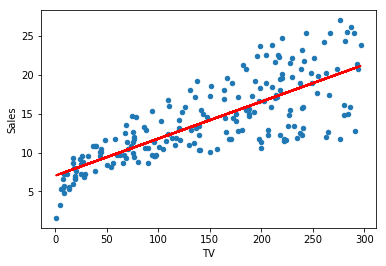
\includegraphics[width=10cm,keepaspectratio=true]{./images/statsModelExample.png}
 % statsModelExample.png: 0x0 pixel, 300dpi, 0.00x0.00 cm, bb=
\end{center}


[]
Ahora calculemos el valor \texttt{RSE}
\begin{lstlisting}[language=Python]
advert['sales_pred']=0.047537*advert['TV']+7.03
advert['RSE']=(advert['Sales']-advert['sales_pred'])**2
SSD=advert.sum()['RSE']
n = len(advert["Sales"])
RSE=np.sqrt(SSD/(n-2))
salesmean=np.mean(advert['Sales'])
error=RSE/salesmean
print(RSE,salesmean,error)
\end{lstlisting}


La salida consta de tres números, el primero de los cuales es $\texttt{RSE} = 3.25$, el segundo es
\texttt{salesmean} (media de ventas reales) $= 14.02$ y \texttt{error} es su proporción, que es igual
a $0.23$.




Por lo tanto, en promedio, este modelo tendrá un $23\%$, incluso si los coeficientes son
correctamente predichos.



Esta es una cantidad significativa de errores y nos gustaría bajarla de alguna manera. Además, se puede mejorar el valor de $R^{2}=0.61$.



Algo que
podemos intentar es agregar más columnas en el modelo, como predictores y ver si mejora el resultado o no.


\section{Regresión lineal múltiple}

Cuando la regresión lineal involucra más de un predictor, entonces es llamada \emph{regresión lineal múltiple}.



La naturaleza del modelo permanece igual, lineal, excepto que puede haber múltiples pendientes $\beta_{i}$ asociadas con cada predictor.




 El modelo se representaría como sigue:
 \begin{align}
 Y = \a + \beta_{1}X_{1}+...+\beta_{n}X_{n}
\end{align}



Cada $\beta_{i}$ se estimará usando el mismo método, \emph{mínimos cuadrados}; por tanto, tendríamos un valor$-p$ asociado con las estimación: 
\begin{enumerate}
 \item Entre más pequeño sea este, más significativo será la variable para el modelo. 
 \item En cambio, las variables con valores$-p$ muy grandes deberán ser eliminadas del mismo.
\end{enumerate}


\paragraph{Pros y contras}
 \begin{enumerate}
  \item Como la regresión lineal múltiple nos da la posibilidad de incluir más variables como predictores, entonces se incrementa la eficiencia del modelo. 

 \item Sin embargo, también incrementa la complejidad del proceso de construcción del modelo, ya que la selección de las variables significativas puede ser tedioso.
 \end{enumerate}


[]{}
Con una base de datos simples de tres predictores, como en el ejemplo de la publicidad, puede haber varios modelos. Estos son:
\begin{enumerate}[Modelo 1:]
 \item \texttt{Ventas$\sim$TV}
 \item \texttt{Ventas$\sim$periódico}
 \item \texttt{Ventas$\sim$radio}
 \item \texttt{Ventas$\sim$TV+radio}
 \item \texttt{Ventas$\sim$TV+periódico}
 \item \texttt{Ventas$\sim$Periódico+radio}
 \item \texttt{Ventas$\sim$TV+radio+periódico}
\end{enumerate}



\begin{rem}
 Un modelos con $n$ posibles predictores, tendrá $2^{n}-1$ posibles modelos. Por tanto, a medida que los predictores se incrementan, la selección se volverá laboriosa.
\end{rem}



Afortunadamente, tenemos algunos lineamientos para filtrar predictores y escoger los más eficientes:
\begin{itemize}
 \item Mantenga las variables con valores$-p$ más bajos y elimine aquellas con valores$-p$ más altos. 
 \item La inclusión de una variable al modelos idealmente debería incrementar el valor $R^{2}.$  Sin embargo, más adelante \emph{ajustaremos} dicho valor para que sea un indicador más confiable.
\end{itemize}


[]{}
Con base en lo anterior, hay dos enfoques para seleccionar los predictores que quedarán en el modelo final:


\paragraph{Selección progresiva}
\begin{enumerate}
 \item En este enfoque, empezamos con modelo vació (sin predictores) y entonces, comenzamos adicionando variables predictoras una por una. 
 \item La variable cuya adición resulte en el modelo con la menos de la suma residual de cuadrados será adicionada primero al modelo. \item Si el valor$-p$ para la variable es suficientemente pequeña y el valor $R^{2}$ (ajustado) crece, el predictor se incluye en el modelo. 
 \item En otro caso, no.
\end{enumerate}


\paragraph{Selección regresiva}
\begin{enumerate}
 \item En este enfoque, empezamos con un modelo que tiene todas las variables predictoras en el modelo y descartamos algunas de ellas.


\item Si el valor$-p$ de una variable predictora es grande y el valor $R^{2}$ (ajustado) decrece, el predictor se descarta del modelo.



\item En otro caso, permanece en el.
\end{enumerate}



Muchos programas estadísticos, incluyendo Python, dan opciones para seleccionar entre los dos enfoques anteriores cuando se implementa una regresión lineal.


Por ahora, agreguemos algunas variables y veamos como cambia el modelo y la eficiencia, de manera que podamos tener un mejor panorama de que está tras el telón cuando estos enfoque se implementan en un programa estadístico.

\subsection{Modelo 2: \texttt{'Sales$\sim$TV+Newspaper'}}

\begin{enumerate}
 \item Nosotros ya hemos visto un modelo suponiendo una relación lineal entre ventas y costos de publicidad en TV, 
 \item Podemos ignorar los otros modelos que consisten de una sola variable.
 %(esto es, el periódico y el radio, ya que tienen coeficientes de correlación pequeños comparados con la TV).
 
 \item Ahora tratemos de agregar más variables al modelo que ya tenemos y veamos como los parámetros cambian su eficiencia.
\end{enumerate}


[]{\texttt{advertisingModel2.py}}
\begin{lstlisting}[language=Python]
import pandas as pd
import statsmodels.formula.api as smf

advert = pd.read_csv("./dataBases/Advertising.csv")
model2=smf.ols(formula='Sales~TV+Newspaper',
               data=advert).fit()
print(model2.params)
print(model2.pvalues)
print(model2.rsquared)
\end{lstlisting}


[,]{}
\begin{lstlisting}[language=Python]
Intercept    5.774948
TV           0.046901
Newspaper    0.044219
dtype: float64
Intercept    3.145860e-22
TV           5.507584e-44
Newspaper    2.217084e-05
dtype: float64
0.645835493829
\end{lstlisting}


Los valores$-p$ para los coeficientes son muy pequeños, lo que sugiere que todos los estimados son significantes.  La ecuación para este modelo será
\begin{align}
 \texttt{Ventas} = 5.77 + 0.046*\texttt{TV} + 0.04*\texttt{Periódico}
\end{align}


El valor $R^{2}$ es $0.6458$, el cuál resulta en una mejora muy pequeña del valor obtenido en el modelo anterior.

[]{}
Los valores pueden ser predichos usando el siguiente retazo de código:
\begin{lstlisting}[language=Python]
sales_pred=model2.predict(advert[['TV','Newspaper']])
print(sales_pred.head())
\end{lstlisting}

[,]{}
\begin{lstlisting}[language=Python]
0    19.626901
1     9.856348
2     9.646055
3    15.467318
4    16.837102
dtype: float64
\end{lstlisting}

[,]{}
Para calcular el valor \texttt{RSE}, utilizamos las siguientes líneas
\begin{lstlisting}[language=Python]
#RSE
import numpy as np
advert['sales_pred']= 5.77 + 0.046901*advert['TV'] + \
                      0.044219*advert['Newspaper']
advert['SSD'] = (advert['Sales']- \
                  advert['sales_pred'])**2
SSD=advert.sum()['SSD']
n = len(advert["Sales"])
print("n",n)
p = 2
RSE=np.sqrt(SSD/(n-p-1))
print("RSE", RSE)
salesmean=np.mean(advert['Sales'])
print("salesmean", salesmean)
error=RSE/salesmean
print("error", error)
\end{lstlisting}

[,]{}
\begin{lstlisting}[language=Python]
n 200
RSE 3.12072391442
salesmean 14.022500000000003
error 0.222551179492
\end{lstlisting}


El valor $RSE$ resulta ser $3.12 (22\%)$, no muy diferente del modelo sólo con la $TV$. En la fórmula, $p=2$ porque es el número de predictores que estamos utilizando en el modelo.

[]
Utilizando la línea de código
\begin{lstlisting}[language=Python]
 print(model2.summary())
\end{lstlisting} obtenemos la siguiente tabla que es el resumen del modelo:


[,]{} \tiny
\begin{lstlisting}[language=Python]

                            OLS Regression Results
==============================================================================
Dep. Variable:                  Sales   R-squared:                       0.646
Model:                            OLS   Adj. R-squared:                  0.642
Method:                 Least Squares   F-statistic:                     179.6
Date:                Fri, 03 Nov 2017   problema (F-statistic):           3.95e-45
Time:                        21:57:12   Log-Likelihood:                -509.89
No. Observations:                 200   AIC:                             1026.
Df Residuals:                     197   BIC:                             1036.
Df Model:                           2
Covariance Type:            nonrobust
==============================================================================
                 coef    std err          t      P>|t|      [0.025      0.975]
------------------------------------------------------------------------------
Intercept      5.7749      0.525     10.993      0.000       4.739       6.811
TV             0.0469      0.003     18.173      0.000       0.042       0.052
Newspaper      0.0442      0.010      4.346      0.000       0.024       0.064
==============================================================================
Omnibus:                        0.658   Durbin-Watson:                   1.969
problema(Omnibus):                  0.720   Jarque-Bera (JB):                0.415
Skew:                          -0.093   problema(JB):                        0.813
Kurtosis:                       3.122   Cond. No.                         410.
==============================================================================

Warnings:
[1] Standard Errors assume that the covariance matrix of the errors is correctly specified.
\end{lstlisting}


Aunque el estadístico$-F$ decrece, el valor$-p$ asociado también lo hace. Pero es solo una mejora marginal al modelo, como podemos ver en el valor $R^{2}.$ De manera que agregar el periódico no mejora sustantivamente el modelo.

\subsection{Modelo 3: \texttt{'Ventas$\sim$TV+Radio'}}

Ahora tratemos de agregar la radio al modelo, en lugar del periódico. El radio tiene la segunda mejor correlación con la variable \texttt{Ventas} en la matriz de correlación que hemos creado anteriormente.  Entonces se espera que existe alguna mejora significativa en el modelo debido a su adición al modelo.  Veamos si esto ocurre o no:

[]{advertisingModel3.py} \tiny
\begin{lstlisting}[language=Python]
#!/usr/bin/env python3
# -*- coding: utf-8 -*-
import pandas as pd
import statsmodels.formula.api as smf

advert = pd.read_csv("./dataBases/Advertising.csv")
model3=smf.ols(formula='Sales~TV+Radio',data=advert).fit()
print(model3.params)
print(model3.pvalues)

a = model3.params[0]
btv = model3.params[1]
bradio = model3.params[2]

advert["sales_pred"] = a + btv * advert["TV"] + \
                        bradio * advert["Radio"]

sales_pred=model3.predict(advert[['TV','Radio']])
print(sales_pred.head())

print(model3.summary())
\end{lstlisting}


[,]{}\tiny
\begin{lstlisting}[language=Python]
#print(model3.params)
Intercept    2.921100
TV           0.045755
Radio        0.187994
dtype: float64

#print(model3.pvalues)
Intercept    4.565557e-19
TV           5.436980e-82
Radio        9.776972e-59
dtype: float64

#print(sales_pred.head())
0    20.555465
1    12.345362
2    12.337018
3    17.617116
4    13.223908
dtype: float64
\end{lstlisting}

[,]{}\tiny
\begin{lstlisting}[language=Python]
#print(model3.summary())
                            OLS Regression Results
==============================================================================
Dep. Variable:                  Sales   R-squared:                       0.897
Model:                            OLS   Adj. R-squared:                  0.896
Method:                 Least Squares   F-statistic:                     859.6
Date:                Sun, 05 Nov 2017   problema (F-statistic):           4.83e-98
Time:                        20:09:44   Log-Likelihood:                -386.20
No. Observations:                 200   AIC:                             778.4
Df Residuals:                     197   BIC:                             788.3
Df Model:                           2
Covariance Type:            nonrobust
==============================================================================
                 coef    std err          t      P>|t|      [0.025      0.975]
------------------------------------------------------------------------------
Intercept      2.9211      0.294      9.919      0.000       2.340       3.502
TV             0.0458      0.001     32.909      0.000       0.043       0.048
Radio          0.1880      0.008     23.382      0.000       0.172       0.204
==============================================================================
Omnibus:                       60.022   Durbin-Watson:                   2.081
problema(Omnibus):                  0.000   Jarque-Bera (JB):              148.679
Skew:                          -1.323   problema(JB):                     5.19e-33
Kurtosis:                       6.292   Cond. No.                         425.
==============================================================================

Warnings:
[1] Standard Errors assume that the covariance matrix of the errors is correctly specified.
\end{lstlisting}


Observemos que el valor $R^{2}$ se ha incrementado considerablemente debido a la adición de la radio al modelo. De la misma manera, el estadístico$-F$ se incrementado considerablemente del último modelo indicando un modelo altamente eficiente.


El valor \texttt{RSE} puede ser calculado usando el mismo método descrito anteriormente:

[,]{\texttt{advertisingModel3.py }(continuación)} \tiny
\begin{lstlisting}[language=Python]
#RSE
import numpy as np

advert['SSD'] = (advert['Sales']- \
                  advert['sales_pred'])**2
SSD=advert.sum()['SSD']
n = len(advert["Sales"])
print("n",n)
p = 2
RSE=np.sqrt(SSD/(n-p-1))
print("RSE", RSE)
salesmean=np.mean(advert['Sales'])
print("salesmean", salesmean)
error=RSE/salesmean
print("error", error)
\end{lstlisting}


[,]{}
\begin{lstlisting}[language=Python]
n 200
RSE 1.68136091251
salesmean 14.022500000000003
error 0.119904504369
\end{lstlisting}


El valor para este modelos es $\approx 1.68 (12\%)$, el cual es mucho mejor que el $22\sim23\%$ de los modelos anteriores.

\subsection{Modelo 3: \texttt{'Ventas$\sim$TV+Radio+Newspaper'}}

\begin{problema}
 Desarrolle un modelo para
 \begin{center}
  \texttt{``Ventas''$\sim$``TV+Radio+Periódico''};
 \end{center}
 haga un análisis de los estadísticos asociados.  Con base en estas observaciones, trata de responde porque el modelo resulta poco beneficiado de la incorporación del predictor ``Periódico''.
\end{problema}


\paragraph{Conclusiones sobre el modelo}
\begin{itemize}
 \item Existe un coeficiente negativo pequeño para el \texttt{periódico}.  Cuando consideramos sólo \texttt{TV} y \texttt{periódico}, el coeficiente de periódico fue significativamente positivo. 
 \item Para este modelo, el estadístico$-F$ ha decrecido considerablemente de $859.6$ a $570.3$. 
 \item Sin embargo, el valor \texttt{RSE} se incremento aunque de manera modesta. 
\end{itemize}
Con todas estas consideraciones, concluimos que la incorporación del \texttt{periódico} al modelo es poco eficiente (¿porqué?).

\subsection{Multicolinealidad}

La \emph{multicolinealidad} es la razón para el desempeño subóptimo del modelo cuando el predictor \texttt{periódico} es añadido al modelo final.

La multicolinealidad alude a la correlación entre los propios predictores del modelo.


Estas son algunas de las señales de este problemalema común encontrado durante la regresión lineal:  Algunas páginas atrás, cuando creamos la \emph{matriz de correlación} para este conjunto de datos, encontramos que existe una correlación importante de $0.35$ entre el radio y el periódico.

Esto significa que el gasto en periódico esta relacionado con el gasto en radio. La relación entre predictores incrementa la variabilidad de los estimados de los coeficientes de las variables predictoras relacionadas.


El estadístico$-t$ para este coeficiente es calculado al dividir el valor promedio por el la \texttt{variabilidad}.  A medida que la variabilidad se incrementa, el valor del estadístico decrementa y entonces el valor$-p$ crece. 

Por lo cual la problemaabilidad de que la hipótesis nula asociada con el estadístico$-F$ sea aceptado se incrementan. Esto reduce la significación del predictor en el modelo.


Por tanto, la colinealidad es un problemalema que debe ser tomado en cuenta.  Para predictores altamente correlacionados, necesitamos hacer un análisis más a fondo con estas variables y ver cuales inclusiones en el modelo lo hacen más eficaz.


Es una buena práctica identificar parejas de predictores con alta correlación, usando la matriz de correlación y verificar el efecto de la multicolinealidad en el modelo.  Las variables responsables deben de ser removidas del modelo: El \emph{factor de inflación de varianza} ( \texttt{VIF}, por sus siglas en inglés) es un método para abordar este problemalema.

\paragraph{\texttt{VIF} (Variance Inflation Factor)}
Es un método para cuantificar el aumento de la variabilidad del estimado del coeficiente de una variable particular debido a la alta correlación entre dos o más predictores.


El cuantificador \texttt{VIF} necesita ser calculado para cada una de las variables y si el valor es muy alto para una en particular, esta debe ser eliminada del modelo.

[]{}
El siguiente es el proceso subyacente para calcular el valor \texttt{VIF}:
\begin{enumerate}
 \item Calcule $X_{i}$ como una función lineal de otras variables predictoras:
 \begin{align}
 X_{i}=\sum_{j\neq i}a_{j}X_{j}
\end{align}
\item Calcule el valor $R^{2}$ para este modelo y denótelo por $R^{2}_{i}.$ El valor \texttt{VIF} para $X_{i}$ está dado por
\begin{align}
 \texttt{VIF}= \dfrac{1}{1-R_{i}^{2}}
\end{align} 
\item
\begin{itemize}
 \item $VIF=1$: Los predictores no están correlacionados.
 \item $1<VIF<5$: Las predictores estás moderadamente correlacionados con otros predictores y pueden seguir siendo parte del modelo.
 \item $5<VIF$: Los predictores están altamente correlacionados y necesitan ser eliminados del modelo.
\end{itemize}

\end{enumerate}



Podemos calcular los valores \texttt{VIF} asociados a cada predictor con el siguiente retazo de código:

[,]{\texttt{VIF.py}}
\begin{lstlisting}[language=Python]
modelN = smf.ols(formula = "Newspaper~TV+Radio", data = advert).fit()
r2N = modelN.rsquared
VIFN = 1/(1-r2N)
print("VIF(Newspaper):", VIFN)

modelT = smf.ols(formula = "TV~Newspaper+Radio", data = advert).fit()
r2T = modelT.rsquared
VIFT = 1/(1-r2T)
print("VIF(TV):", VIFT)

modelR = smf.ols(formula = "Radio~TV+Newspaper", data = advert).fit()
r2R = modelR.rsquared
VIFR = 1/(1-r2R)
print("VIF(Radio):", VIFR)
\end{lstlisting}

[,]{}
Del cual obtenemos los siguientes resultados
\begin{lstlisting}[language=Python]
VIF(Newspaper): 1.14518737872
VIF(TV): 1.00461078494
VIF(Radio): 1.14495191711
\end{lstlisting}


Los predictores \texttt{Newpaper} y \texttt{Radio} tienen prácticamente los mismos valores \texttt{VIF}, indicando que están correlacionados uno con el otro y no así con el predictor \texttt{TV}.


En este caso, la radio y el periódico están fuertemente correlacionados. Sin embargo, el modelo con \texttt{TV} y \texttt{Radio} como predictores es mucho mejor que aquel con \texttt{TV} y \texttt{Newspaper} como tales.


El modelo con las tres variables como predictores no mejora mucho el modelo. De hecho, incrementa la variabilidad y el estadístico$-F.$


Parece adecuado abandonar el predictor \texttt{Newpaper} del modelo y escoger el modelo 3 como el mejor candidato para el modelo final:
\begin{align}
 \texttt{Ventas} = 2.92 + 0.45*\texttt{TV} + 0.18*\texttt{Radio}
\end{align}


\section{Validación del modelo}

Cualquier modelo predictivo necesita ser validado para observar como es su rendimiento en diferentes conjuntos de datos  y determinar si la precisión del modelo es contante todas fuentes de datos similares o no.


Esto nos ayuda a detectar algún \texttt{problemalema del exceso de ajuste (over-fitting)}, en el que el modelo se ajusta
muy bien en un conjunto de datos, pero no encaja bien en otro conjunto de datos. Un método común es crear un modelo diviendo los datos en categorías de \texttt{entrenamiento/prueba}. Otro método es
\texttt{validación cruzada de $k$ iteraciones}, sobre la cual aprenderemos más en el capítulo posterior.

\subsection{División entre datos de entrenamiento y prueba}

Idealmente, este paso debería hacerse justo al inicio del proceso de modelado para que
no haya sesgos de muestreo en el modelo; en otras palabras, el modelo debería funcionar
bien incluso para un conjunto de datos que tiene las mismas variables de predicción, pero sus medias y
las varianzas son muy diferentes sobre de las que se ha construido el modelo.


Esto puede
suceder porque el conjunto de datos en el que se basa el modelo (entrenamiento o capacitación) y el de
que se aplica (prueba) puede provenir de diferentes fuentes. Una forma más robusta de
hacer esto es un proceso llamado la validación cruzada de $k$ iteraciones, sobre la cual hablaremos en
detalle en un momento.


Veamos cómo podemos dividir el conjunto de datos disponible en el conjunto de datos de entrenamiento y prueba
y aplicar el modelo al conjunto de datos de prueba para obtener otros resultados:

[,]{\texttt{crossValidation.py}}
\begin{lstlisting}[language=Python]
import pandas as pd
import statsmodels.formula.api as smf

advert = pd.read_csv("./dataBases/Advertising.csv")
model3=smf.ols(formula='Sales~TV+Radio',data=advert).fit()
sales_pred=model3.predict(advert[['TV','Radio']])
print(sales_pred.head())

print(model3.summary())

import numpy as np

N = len(advert)
arr =  np.arange(N)
np.random.shuffle(arr)
check = arr < 0.8*N
training=advert[check].copy()
testing=advert[~check].copy()
\end{lstlisting}


Vamos a crear un modelo para entrenar los datos y problemaar el rendimiento del modelo en
datos de prueba. Creemos el único modelo que funciona mejor (lo hemos encontrado ya),
el que tiene variables de TV y radio, como variables de predicción:

[,]{}
\begin{lstlisting}[language=Python]
import statsmodels.formula.api as smf
model5=smf.ols(formula='Sales~TV+Radio',data=training).fit()
print(model5.summary())
\end{lstlisting}

[,]{\texttt{print(model3.summary())}}
\tiny
\begin{lstlisting}[language=Python]
                            OLS Regression Results
==============================================================================
Dep. Variable:                  Sales   R-squared:                       0.897
Model:                            OLS   Adj. R-squared:                  0.896
Method:                 Least Squares   F-statistic:                     859.6
Date:                Sun, 12 Nov 2017   problema (F-statistic):           4.83e-98
Time:                        22:40:26   Log-Likelihood:                -386.20
No. Observations:                 200   AIC:                             778.4
Df Residuals:                     197   BIC:                             788.3
Df Model:                           2
Covariance Type:            nonrobust
==============================================================================
                 coef    std err          t      P>|t|      [0.025      0.975]
------------------------------------------------------------------------------
Intercept      2.9211      0.294      9.919      0.000       2.340       3.502
TV             0.0458      0.001     32.909      0.000       0.043       0.048
Radio          0.1880      0.008     23.382      0.000       0.172       0.204
==============================================================================
Omnibus:                       60.022   Durbin-Watson:                   2.081
problema(Omnibus):                  0.000   Jarque-Bera (JB):              148.679
Skew:                          -1.323   problema(JB):                     5.19e-33
Kurtosis:                       6.292   Cond. No.                         425.
==============================================================================

Warnings:
[1] Standard Errors assume that the covariance matrix of the errors is correctly specified.
\end{lstlisting}

[,]{}
\tiny
\begin{lstlisting}[language=Python]
                            OLS Regression Results
==============================================================================
Dep. Variable:                  Sales   R-squared:                       0.906
Model:                            OLS   Adj. R-squared:                  0.904
Method:                 Least Squares   F-statistic:                     753.7
Date:                Sun, 12 Nov 2017   problema (F-statistic):           3.22e-81
Time:                        22:40:26   Log-Likelihood:                -299.60
No. Observations:                 160   AIC:                             605.2
Df Residuals:                     157   BIC:                             614.4
Df Model:                           2
Covariance Type:            nonrobust
==============================================================================
                 coef    std err          t      P>|t|      [0.025      0.975]
------------------------------------------------------------------------------
Intercept      2.8708      0.318      9.035      0.000       2.243       3.498
TV             0.0448      0.001     30.797      0.000       0.042       0.048
Radio          0.1959      0.009     22.803      0.000       0.179       0.213
==============================================================================
Omnibus:                       11.888   Durbin-Watson:                   2.158
problema(Omnibus):                  0.003   Jarque-Bera (JB):               13.175
Skew:                          -0.696   problema(JB):                      0.00138
Kurtosis:                       2.807   Cond. No.                         438.
==============================================================================

Warnings:
[1] Standard Errors assume that the covariance matrix of the errors is correctly specified.
\end{lstlisting}


La mayoría de los parámetros del modelo, como la intercepción, las estimaciones de coeficientes y $R^2$ son
muy similares.


La diferencia en el estadístico$-F$ se puede atribuir a un conjunto de datos más pequeño. Cuanto menor sea el conjunto de datos, mayor será el valor de \texttt{SSD} y menor será el valor de
el término $(n-p-1)$ en la fórmula del estadístico$-F$; ambos contribuyen a la disminución en el valor estadístico$-F.$


El modelo puede reescribirse como sigue:
\begin{align}
 \texttt{Ventas} \sim 2.86 + 0.04*\texttt{TV} + 0.17*\texttt{Radio}
\end{align}

[,]{}
Ahora, predigamos los valores de las ventas para los valores de prueba:
\tiny
\begin{lstlisting}[language=Python]
sales_pred=model5.predict(training[['TV','Radio']])
sales_pred
\end{lstlisting}


El valor \texttt{RSE} para esta predicción en el conjunto de datos de prueba puede ser calculadas usando el siguiente pedazo de código:

[,]{}
\begin{lstlisting}[language=Python]
testing['sales_pred']=2.86 + 0.04*testing['TV'] + 0.17*testing['Radio']
n = len(testing)
p = 2
testing['SSD']=(testing['Sales']-testing['sales_pred'])**2
SSD=testing.sum()['SSD']
RSE=np.sqrt(SSD/(n-p-1))
salesmean=np.mean(testing['Sales'])
error=RSE/salesmean
print(RSE,salesmean,error)
##2.33080393856 14.527500000000003 0.160440814907
\end{lstlisting}


El valor \texttt{RSE} resulta ser $2.54$ sobre una venta promedio (en el conjunto de datos) de $14.80$, lo cual es un error del $17\%$.


Podemos ver que el modelo no se generaliza muy bien en el conjunto de datos de prueba, ya que el valor \texttt{RSE} para el mismo modelo es diferente en los dos casos.


Implica un cierto grado de exceso de ajuste cuando tratamos de construir el modelo basado en todo el conjunto de datos.


El valor \texttt{RSE} con
la división de pruebas de entrenamiento, aunque un poco mayor, es más confiable y replicable.

\section{Resumen de modelos}

\begin{figure}
 \centering
 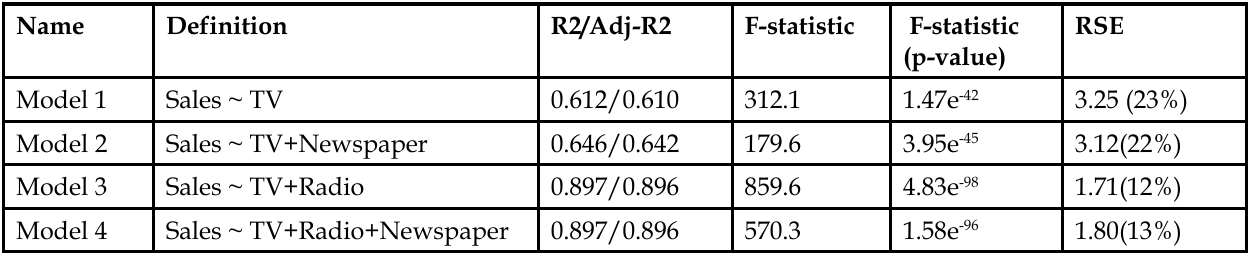
\includegraphics[width=10cm,keepaspectratio=true]{./images/modelsGuide.png}
 % modelsGuide.png: 0x0 pixel, 300dpi, 0.00x0.00 cm, bb=
 \caption{Guía para la selección de variables.}
 \label{fig:modelsGuide}
\end{figure}


[]{}
Finalmente, para resumir, para un buen modelo lineal, los predictores deberían escogerse con base en los siguientes criterios:
\begin{itemize}
 \item \texttt{$R^2$}: Este valor siempre aumentará cuando se agregue una nueva variable de predicción al
modelo. Sin embargo, no es una verificación muy confiable de la mayor eficiencia de
el modelo. Más bien, para un modelo eficiente, debemos verificar el $R^2$ ajustado.
Esto debería aumentar al agregar una nueva variable de predicción.
\item \texttt{valor$-p$}: Cuanto menor sea el valor$-p$ para la estimación de la variable de predicción,
mejor es agregar la variable de predicción al modelo.
\item \texttt{Estadístico$-F$}: El valor del estadístico$-F$ para el modelo debería aumentar después de
la adición de una nueva variable de predicción para considerarse una
adición eficiente al modelo. El aumento en el estadístico$-F$ es un buen indicador para la mejora en el modelo debida únicamente por la adición de ese variable particular. Alternativamente, el valor$-p$ asociado con el estadístico $F$ debería disminuir al agregar una nueva variable de predicción. 
\item \texttt{RSE}: Este valor para el nuevo modelo debería disminuir al agregar
la nueva variable de predicción.
\item \texttt{VIF}: Para ocuparse de los Problemas que surgen debido a la colinealidad múltiple, se necesita
eliminar las variables con grandes valores \texttt{VIF}.
\end{itemize}


\section{Regresión lineal con \texttt{scikit-learn}}

Vamos a implementar el modelo de regresión lineal utilizando el paquete \texttt{scikit-learn}. Este método es más elegante ya que tiene más métodos incorporados para realizar
los procesos regulares asociados con la regresión.


Por ejemplo, podrías recordar
del último capítulo que hay un método separado para dividir el conjunto de datos en
entrenamiento y prueba de conjuntos de datos:

[,]{\texttt{scikitExample.py}}
\begin{lstlisting}[language=Python]
advert = pd.read_csv("./dataBases/Advertising.csv")
feature_cols = ['TV', 'Radio']
X = advert[feature_cols]
Y = advert['Sales']
trainX,testX,trainY,testY = train_test_split(X,Y, test_size = 0.2)
lm = LinearRegression()
lm.fit(trainX, trainY)
\end{lstlisting}

[,]{}
El siguiente código nos devuelve los parámetros
\begin{lstlisting}[language=Python]
print(lm.intercept_)
for _ in zip(feature_cols, lm.coef_):
    print(_)
\end{lstlisting}

[,]{}
El valor $R^{2}$ se obtiene de la siguiente manera
\begin{lstlisting}[language=Python]
print("R2 =", lm.score(trainX, trainY))
\end{lstlisting}

[,]{}
Un resultado típico de este código sería
\begin{lstlisting}[language=Python]
2.73465274245
('TV', 0.046830472078714387)
('Radio', 0.18642021416992249)
R2 = 0.893905959809
\end{lstlisting}


Los valores de $R^{2}$ resultan alrededor del $89\%,$ muy cercanos al valor obtenido por el método usado anteriormente.

[,]{}
El modelo puede ser usado para predecir el valor de las ventas usando los predictores \texttt{TV} y \texttt{Radio} del conjunto de datos de prueba, como sigue:
\begin{lstlisting}[language=Python]
lm.predict(testX)
\end{lstlisting}


\subsection{Selección de características con \texttt{scikit-learn}}

Muchas de las herramientas y paquetes estadísticos tienen métodos incorporados para
llevar a cabo un proceso de selección de variables (selección hacia adelante y selección hacia atrás).


Si
se hace manualmente, consumirá mucho tiempo y seleccionar los más importantes  variables serán una tarea tediosa que compromete la eficiencia del modelo.


Una ventaja de usar el paquete \texttt{scikit-learn} para la regresión en Python es
que tiene este método particular para la selección de características. Esto funciona más o menos como
selección hacia atrás (no exactamente) y se llama \texttt{eliminación de características recursivas}, (\texttt{RFE}, por sus siglas en inglés).
Se puede especificar el número de variables que desean en el modelo final.


El modelo se ejecuta primero con todas las variables y se asignan ciertos pesos a todos
las variables. En las iteraciones siguientes, las variables con los pesos más pequeños
se borran de la lista de variables hasta que se deja el número deseado de variables.


Veamos cómo se puede hacer una selección de funciones en \texttt{scikit-learn}:

[,]{\texttt{RFE.py}}
\begin{lstlisting}[language=Python]
import pandas as pd
advert = pd.read_csv("./dataBases/Advertising.csv")

from sklearn.feature_selection import RFE
from sklearn.svm import SVR
feature_cols = ['TV', 'Radio','Newspaper']
X = advert[feature_cols]
Y = advert['Sales']
estimator = SVR(kernel="linear")
selector = RFE(estimator,2,step=1)
selector = selector.fit(X, Y)
\end{lstlisting}


Usamos los métodos denominados \texttt{RFE} y \texttt{SVR} integrados en \texttt{scikit-learn}. Indicamos que
queremos estimar un modelo lineal y que el número de variables deseadas en el modelo son dos.

[,]{}
Para obtener la lista de variables seleccionadas, uno puede escribir el siguiente fragmento de código:
\begin{lstlisting}[language=Python]
print(selector.support_)
##[ True  True False]
\end{lstlisting}


En nuestro caso, \texttt{X} consta de tres variables: \texttt{TV}, \texttt{Radio} y \texttt{Newpaper}. La matriz anterior sugiere que la TV y la radio se han seleccionado para el modelo, mientras que
el periódico no ha sido seleccionado. Esto concuerda con la selección de variables que tuvimos hecho manualmente

[]
Este método también devuelve una clasificación, como se describe en el siguiente ejemplo:
\begin{lstlisting}[language=Python]
print(selector.ranking_)
##[1 1 2]
\end{lstlisting}



\begin{rem}
 Todas las variables seleccionadas tendrán una clasificación de 1 mientras que las siguientes serán
clasificadas en orden descendente respecto de su importancia. Una variable con rango 2 será más
significativa para el modelo que la que tiene un rango de 3 y así sucesivamente.
\end{rem}



\section{Manejando otros Problemas en lineales regresión}

Hasta ahora en este capítulo, hemos aprendido:
\begin{itemize}
 \item Cómo implementar un modelo de regresión lineal usando dos métodos
 \item Cómo medir la eficiencia del modelo usando los parámetros del modelo
\end{itemize}


Sin embargo, hay otros Problemas que deben tenerse en cuenta al tratar con fuentes de datos de diferentes tipos. Repasemos uno por uno. Usaremos un diferente conjunto de datos simulado para ilustrar estos Problemas. Vamos a importarlo y echarle un vistazo
en eso:

[,]{\texttt{handlingIssues.py}}
\begin{lstlisting}[language=Python]
import pandas as pd
df=pd.read_csv('./dataBases/EcomExpense.csv')
print(df.head())
\end{lstlisting}

[,]{}
Deberíamos obtener los siguientes resultados:
\tiny
\begin{lstlisting}[language=Python]
  Transaction ID  Age    Items   Monthly Income  Transaction Time  Record  \
0         TXN001    42       10            7313        627.668127       5
1         TXN002    24        8           17747        126.904567       3
2         TXN003    47       11           22845        873.469701       2
3         TXN004    50       11           18552        380.219428       7
4         TXN005    60        2           14439        403.374223       2

   Gender City Tier  Total Spend
0  Female    Tier 1  4198.385084
1  Female    Tier 2  4134.976648
2    Male    Tier 2  5166.614455
3  Female    Tier 1  7784.447676
4  Female    Tier 2  3254.160485
\end{lstlisting}

[]{}
La captura de pantalla anterior es un conjunto de datos simulados del sitio web de cualquier comercio. Esto captura la información sobre varias transacciones realizadas en el sitio web.


Una breve
La descripción de los nombres de columna del conjunto de datos es la siguiente:
\begin{itemize}
 \item Identificación de transacción: ID de transacción para la transacción
\item Edad: Edad del cliente
\item Artículos: número de artículos en el carrito de compras (comprado)
\item Ingreso mensual: Ingreso disponible mensual del cliente
\item Tiempo de transacción: tiempo total pasado en el sitio web durante la transacción
\item Registro: cuántas veces el cliente ha comprado con el sitio web en
el pasado
\item Género: Género del cliente
\item Nivel de la ciudad: ~
\item Gasto total: monto total gastado en la transacción
\end{itemize}



La variable de salida es la variable\texttt{Total Spend (Gasto total)}. Los otros son predictores potenciales
variables y sospechamos que el gasto total está relacionado linealmente con todos estos
variables predictoras.


\subsection{Manejando variables categóricas}

Hasta ahora, hemos supuesto que las variables de predicción solo pueden ser cuantitativas o
numéricas, pero sabemos por experiencias de la vida real que la mayoría de las veces \emph{el conjunto de datos
contiene una variable categórica o cualitativa} y muchas de las veces estas variables
tendrá un impacto significativo en el valor de la salida. Sin embargo, la pregunta es
\emph{¿cómo procesar estas variables, para usarlas en el modelo?}


No podemos asignarles valores, como 0, 1, 2, etc., y luego usarlos en el
modelo, ya que dará un peso excesivo a las categorías debido a los números
asignado a ellos. 

La mayoría de las veces puede dar un resultado incorrecto y cambiará,
como cambia el número asignado a una categoría en particular.


En el marco de datos que acabamos de importar, Género y Nivel de ciudad son los categóricos
variables.


Para manejar variables categóricas, usaremos variables ``tontas'' (dummies, en inglés) o ficticias.


Una regresión lineal es de la forma
\begin{align}
 Y_{\texttt{model}}=\a + \sum \beta_{i}X_{i}
\end{align}
en la cual algunas $X_{i}$ pueden ser categóricas. Digamos que $X_{g}$ es tal variable.


En nuestro ejemplo,
\begin{align}X_{g}=
 \begin{cases}
  1 & \texttt{cliente masculino} \\
  0 & \texttt{cliente femenino}
 \end{cases}
\end{align}


Si hay tres niveles en la variable categórica, entonces uno necesita definir dos
variables en comparación con 1 cuando había dos niveles en la variable categórica.

Por ejemplo, la variable \texttt{City Tier} tiene tres niveles en nuestro conjunto de datos.


Para esto, podemos definir dos variables, tales que:
\begin{align}
 X_{t1}=
 \begin{cases}
  1 & \texttt{``City Tier''}=1 \\
  0 & \texttt{``City Tier''}\neq 1
 \end{cases}
 \end{align}
 \begin{align}
 X_{t2}=
 \begin{cases}
  1 & \texttt{``City Tier''}=2 \\
  0 & \texttt{``City Tier''}\neq 2
 \end{cases}
\end{align}


Entonces, el modelo puede ser alguno de los siguientes
\begin{align}
 Y=
 \begin{cases}
  \a + \beta_{1}X_{1}+...+\beta_{t1}X_{t1}+...+b_{n}X_{n} & \texttt{``City Tier''=1}\\
  \a + \beta_{1}X_{1}+...+\beta_{t1}X_{t2}+...+b_{n}X_{n} & \texttt{``City Tier''=2}\\
  \a + \beta_{1}X_{1}+...++b_{n}X_{n} & \texttt{``City Tier''=3}\\
 \end{cases}
\end{align}


Tengan en cuenta que uno no tiene que crear la tercera variable. Esto es
debido a la naturaleza en que se definen estas variables.


Si un
el cliente no pertenece a la ciudad de nivel 1 o nivel 2, entonces ciertamente lo hará
pertenece a una ciudad de nivel 3. Por lo tanto, no se requiere una variable para uno de
los niveles.


\begin{rem}
 En general, para variables categóricas que tienen $n$ niveles, uno
debería crear $(n-1)$ variables ficticias.
\end{rem}

Sin embargo, por simplicidad, utilizaremos cada uno de los niveles.


Creemos ahora las variables ficticias para nuestras
variables categóricas y luego agreguémoslas a nuestro marco de datos, como se muestra:


[,]{}
\tiny
\begin{lstlisting}[language=Python]
dummy_gender=pd.get_dummies(df['Gender'],prefix='Sex')
dummy_city_tier=pd.get_dummies(df['City Tier'],prefix='City')
\end{lstlisting}


Veamos cómo se ven y si satisfacen las condiciones que hemos definido
antes o no. Así es como se ve \texttt{dummy\_city\_tier}:

[,]{}
\begin{lstlisting}[language=Python]
   City_Tier 1  City_Tier 2  City_Tier 3
0            1            0            0
1            0            1            0
2            0            1            0
3            1            0            0
4            0            1            0
\end{lstlisting}

[,]{}
\texttt{dummy\_gender} es similar a la siguiente tabla:
\begin{lstlisting}[language=Python]
   Sex_Female  Sex_Male
0           1         0
1           1         0
2           0         1
3           1         0
4           1         0
\end{lstlisting}


Ahora, tenemos estas variables ficticias creadas pero no son parte del
marco principal de datos todavía. Vamos a adjuntar estas nuevas variables al marco de datos principal para que
se puede usar en el modelo:

[,]{}
\tiny
\begin{lstlisting}[language=Python]
  Transaction ID  Age    Items   Monthly Income  Transaction Time  Record  \
0         TXN001    42       10            7313        627.668127       5
1         TXN002    24        8           17747        126.904567       3
2         TXN003    47       11           22845        873.469701       2
3         TXN004    50       11           18552        380.219428       7
4         TXN005    60        2           14439        403.374223       2

   Gender City Tier  Total Spend  Sex_Female  Sex_Male  City_Tier 1  \
0  Female    Tier 1  4198.385084           1         0            1
1  Female    Tier 2  4134.976648           1         0            0
2    Male    Tier 2  5166.614455           0         1            0
3  Female    Tier 1  7784.447676           1         0            1
4  Female    Tier 2  3254.160485           1         0            0

   City_Tier 2  City_Tier 3
0            0            0
1            1            0
2            1            0
3            0            0
4            1            0
\end{lstlisting}


Hay cinco nuevas columnas en el marco de datos, dos de las variables ficticia de \texttt{Gender} y tres de las variables ficticias de \texttt{City Level}.


Si lo compara con el conjunto de datos completo, \texttt{City\_Tier\_1} tiene el valor 1 si \texttt{City\_Tier}
tiene valor de \texttt{Tier 1}, \texttt{City\_Tier\_2} tiene valor 1 si \texttt{City\_Tier} tiene valor de \texttt{Tier 2} y
\texttt{City\_Tier\_3} tiene valor 1 si \texttt{City\_Tier} tiene valor \texttt{Tier 3}. Todas las demás variables ficticias en esa fila particular tendrán valores 0. Esto es lo que queríamos.


Veamos cómo incluir estas variables ficticias en el modelo y cómo evaluarlas
sus coeficientes.

Para el conjunto de datos anterior, supongamos una relación lineal entre la salida
variable de Gasto Total y las variables predictoras: \texttt{Ingreso Mensual} y
\texttt{Tiempo de transacción}, y ambos conjuntos de variables ficticias:

[,]{}
\tiny
\begin{lstlisting}[language=Python]
from sklearn.linear_model import LinearRegression
feature_cols = ['Monthly Income','Transaction Time','City_Tier 1',\
                'City_Tier 2','City_Tier 3','Sex_Female','Sex_Male']
X = df2[feature_cols]
Y = df2['Total Spend']
lm = LinearRegression()
lm.fit(X,Y)
\end{lstlisting}

[,]{}
Los parámetros del modelo se pueden encontrar de la siguiente manera:
\begin{lstlisting}[language=Python]
print(lm.intercept_)
for _ in zip(feature_cols, lm.coef_):
    print(_)
\end{lstlisting}

[,]{}
\begin{lstlisting}[language=Python]
3655.72940769
('Monthly Income', 0.15297824609320512)
('Transaction Time', 0.12372608642619998)
('City_Tier 1', 119.66325160390086)
('City_Tier 2', -16.67901800799039)
('City_Tier 3', -102.9842335959104)
('Sex_Female', -94.157798830320132)
('Sex_Male', 94.157798830320118)
\end{lstlisting}

[,]{}
El valor $R^2$ para este modelo se puede encontrar escribiendo lo siguiente:
\begin{lstlisting}[language=Python]
R2 = lm.score(X,Y)
print(R2)
## 0.194789205529
\end{lstlisting}


El valor resulta ser $0.19$, lo que podría deberse a que no hemos usado las otras variables y el resultado también podrían estar relacionados con ellos. 

Necesitamos ajustar el
modelo al transformar adecuadamente algunas de las variables y agregarlas al modelo. 

Por ejemplo, si agregamos la variable \texttt{Record} al modelo, $R^2$ salta a $0.91$ (intente eso
por su cuenta). Es un buen conjunto de datos para jugar.

El modelo se puede escribir de la siguiente manera:
\begin{align}
\texttt{Total\_Spend}= & 3655.72+0.12*\texttt{Transaction Time} \\ &+0.15*\texttt{Monthly Income}+119*\texttt{City\_Tier 1}\\
& -16*\texttt{City\_Tier 2} - 102*\texttt{City\_Tier 3}\\
& -94*\texttt{Sex\_Female}+94*\texttt{Sex\_Male}
\end{align}

[,]{}
El RSE se puede calcular de la siguiente manera:
\tiny
\begin{lstlisting}[language=Python]
import numpy as np
df2['total_spend_pred']=3720.72940769 + 0.12*df2['Transaction Time']+ \
    0.15*df2['Monthly Income']+119*df2['City_Tier 1']-16*df2['City_Tier 2']
-102*df2['City_Tier 3']-94*df2['Sex_Female']+94*df2['Sex_Male']
df2['RSE']=(df2['Total Spend']-df2['total_spend_pred'])**2
RSEd=df2.sum()['RSE']
RSE=np.sqrt(RSEd/2354)
salesmean=np.mean(df2['Total Spend'])
error=RSE/salesmean
print(RSE,salesmean,error)
##2518.85203887 6163.176415976714 0.408693808008
\end{lstlisting}


Para diferentes niveles de género y ciudad, el modelo se reducirá a seguir para
diferentes casos:
\begin{center}
 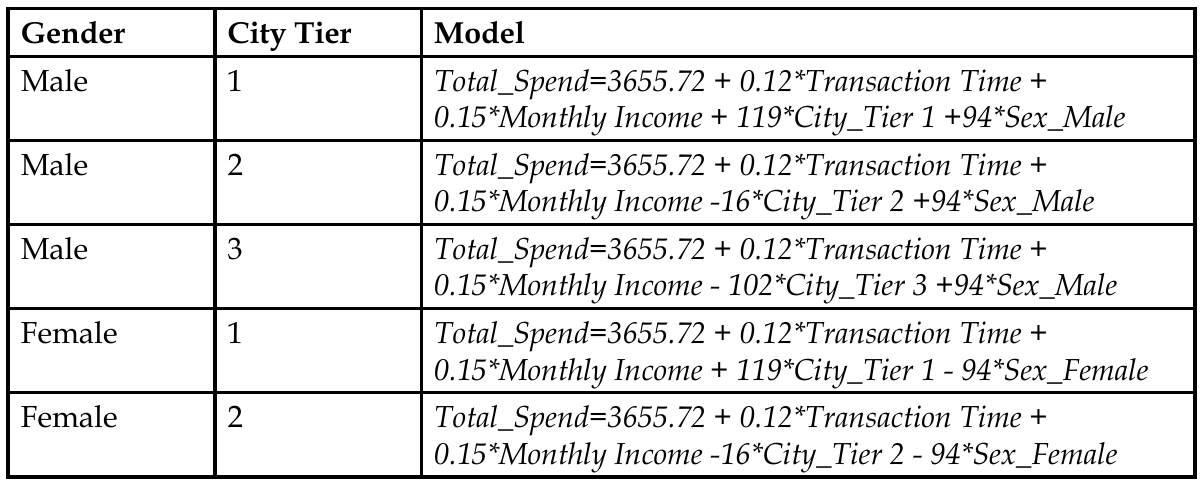
\includegraphics[width=10cm,keepaspectratio=true]{./images/dummies.png}
 % dummies.png: 0x0 pixel, 300dpi, 0.00x0.00 cm, bb=
\end{center}



\subsection{Transformando una variable para ajustarla a una relación no lineal}

A veces, la variable de salida no tiene una relación lineal directa con el
variable de predicción, es decir, tienen una relación no lineal.


Estas relaciones podrían
funciones simples como cuadrática, exponencial, logaritmo o complejas como
polinomios. En tales casos, la transformación de la variable es muy útil.


La siguiente es una guía aproximada sobre cómo hacerlo:
\begin{enumerate}
 \item
 Trace un diagrama de dispersión de la variable de salida con cada uno de los predictores
variables. Este se puede pensar como una matriz de diagrama de dispersión similar a
la matriz de correlación
\item Si la gráfica de dispersión asume más o menos una forma lineal para una variable de predicción
entonces está relacionado linealmente con la variable de salida.
\item Si el diagrama de dispersión asume una forma característica de diferente de la lineal para una variable de predicción, entonces transformaremos esa variable en particular
aplicando esa función.
\end{enumerate}


Vamos a ilustrar esto con un ejemplo. Usaremos el conjunto de datos \texttt{Auto.csv} para esto.
Este conjunto de datos contiene información sobre millas por galón (mpg) y caballos de fuerza para
una serie de modelos de automóviles y mucho más. El \texttt{mpg} es la variable de predicción y es
considerado altamente dependiente de la potencia de un modelo de automóvil.

[,]{\texttt{nonLinear.py}}
\begin{lstlisting}[language=Python]
import pandas as pd
data = pd.read_csv('./dataBases/Auto.csv')
print(data.head())
\end{lstlisting}

[,]{}
\tiny
\begin{lstlisting}[language=Python]
    mpg  cylinders  displacement  horsepower  weight  acceleration  \
0  18.0          8         307.0       130.0    3504          12.0
1  15.0          8         350.0       165.0    3693          11.5
2  18.0          8         318.0       150.0    3436          11.0
3  16.0          8         304.0       150.0    3433          12.0
4  17.0          8         302.0       140.0    3449          10.5

   model year  origin                   car name
0          70       1  chevrolet chevelle malibu
1          70       1          buick skylark 320
2          70       1         plymouth satellite
3          70       1              amc rebel sst
4          70       1                ford torino
\end{lstlisting}


Tiene 406 filas y 9 columnas. Algunas de las variables tienen valores de \texttt{NA (not available)} y tiene sentido eliminar los valores \texttt{NA} antes de usarlos.

[,]{}
Ahora, tracemos un diagrama de dispersión entre las variables de potencia y \texttt{mpg} para ver
ya sea que exhiban una forma lineal o alguna forma no lineal:
\begin{lstlisting}[language=Python]
import matplotlib.pyplot as plt
#%matplotlib inline
data['mpg']=data['mpg'].dropna()
data['horsepower']=data['horsepower'].dropna()
plt.plot(data['horsepower'],data['mpg'],'ro')
plt.xlabel('Horsepower')
plt.ylabel('MPG (Miles Per Gallon)')
\end{lstlisting}


\begin{figure}
 \centering
 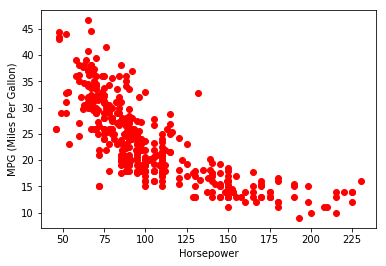
\includegraphics[width=10cm,keepaspectratio=true]{./images/hpVsMpg.png}
 % hpVsMpg.png: 0x0 pixel, 300dpi, 0.00x0.00 cm, bb=
 \caption{\texttt{HP vs MPG}}
 \label{fig:hp}
\end{figure}


Aunque hemo supuesto que el modelo es lineal
\begin{align}
 mpg = c_{0} + c_{1}*\texttt{hp}
\end{align}
en realidad parece más un \emph{modelo cuadrático}
\begin{align}
 mpg = c_{0} + c_{1}*\texttt{hp} + c_{2}\texttt{hp}^{2}
\end{align}


El siguiente fragmento de código se ajustará a un modelo lineal entre potencia y mpg
variables. Los valores de NA deben eliminarse de las variables antes de que puedan
ser utilizado en el modelo. También simultáneamente, creemos un modelo asumiendo un lineal
relación entre mpg y cuadrado de potencia:

[,]{}
\begin{lstlisting}[language=Python]
import numpy as np
from sklearn.linear_model import LinearRegression
X=data['horsepower'].fillna(data['horsepower'].mean())
Y=data['mpg'].fillna(data['mpg'].mean())
lm=LinearRegression()
lm.fit(X[:,np.newaxis],Y)
\end{lstlisting}


El método de regresión lineal por defecto requiere que X sea una matriz de dos
dimensiones. Usando \texttt{np.newaxis}, estamos creando una nueva dimensión para que
funcione correctamente.

La línea de mejor ajuste se puede trazar con el siguiente fragmento:

[,]{}
\begin{lstlisting}[language=Python]
import matplotlib.pyplot as plt
%matplotlib inline
plt.plot(data['horsepower'],data['mpg'],'ro')
plt.plot(X,lm.predict(X[:,np.newaxis]),color='blue')
\end{lstlisting}



\begin{center}
 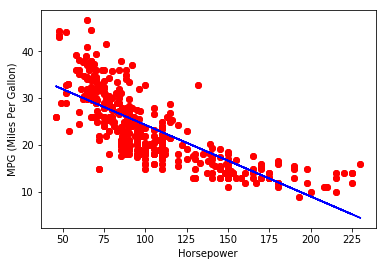
\includegraphics[width=10cm,keepaspectratio=true]{./images/hpLR.png}
 % hpLR.png: 0x0 pixel, 300dpi, 0.00x0.00 cm, bb=
\end{center}
[,]{}
\begin{lstlisting}[language=Python]
R2 = lm.score(X[:,np.newaxis],Y)
print(R2)
## 0.574653340645

RSEd=(Y-lm.predict(X[:,np.newaxis]))**2
RSE=np.sqrt(np.sum(RSEd)/389)
ymean=np.mean(Y)
error=RSE/ymean
print(RSE,error)
## 5.1496254787 0.21899719414
\end{lstlisting}


Aquí, estamos usando el método \texttt{predict} para calcular el valor predicho de la
modelo en lugar de escribirlos explícitamente.

El valor de RSE para este modelo resulta ser 5.14, que sobre un valor medio de 23.51 da un error del 21\%



Si el modelo es cuadrático, esto se puede ajustar utilizando el método \texttt{PolynomialFeatures} en la biblioteca \texttt{scikit-learn}. En este modelo, asumimos una relación polinómica entre mpg
y caballos de fuerza:

[,]{\texttt{nonLinear.py}}
\begin{lstlisting}[language=Python]
from sklearn.preprocessing import PolynomialFeatures
from sklearn import linear_model
X=data['horsepower'].fillna(data['horsepower'].mean())
Y=data['mpg'].fillna(data['mpg'].mean())
poly = PolynomialFeatures(degree=2)
X_ = poly.fit_transform(X[:,np.newaxis])
clf = linear_model.LinearRegression()
clf.fit(X_, Y)

print(clf.intercept_)
##55.0261924471
print(clf.coef_)
##[ 0.         -0.43404318  0.00112615]
\end{lstlisting}


El modelo se puede escribir entonces como
\begin{align}
 \texttt{mpg}  = 55.02 -0.43*\texttt{hp}+0.001*\texttt{hp}^{2}
\end{align}

[,]{}
Con el siguiente fragmento de código, podemos visualizar el modelo cuadrático:
\begin{lstlisting}[language=Python]
plt.plot(data['horsepower'],data['mpg'],'ro')
plt.plot(X,clf.predict(X_), "bo")
plt.show()
\end{lstlisting}


\begin{center}
 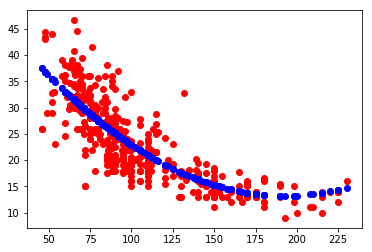
\includegraphics[width=10cm,keepaspectratio=true]{./images/hpNLR.png}
 % hpNLR.png: 0x0 pixel, 300dpi, 0.00x0.00 cm, bb=
\end{center}


